\documentclass[10pt, a4paper,spanish]{article}

\usepackage[utf8]{inputenc}
\usepackage[spanish]{babel}

\usepackage[T1]{fontenc}

\usepackage[hmarginratio=1:1,top=32mm,columnsep=20pt]{geometry}
\usepackage[hang, small,labelfont=bf,up,textfont=it,up]{caption}

\usepackage{float}

\usepackage{amsmath}

\usepackage{graphicx}
\graphicspath{ {images/} }


\usepackage{titlesec}
\renewcommand\thesection{\Roman{section}}
\renewcommand\thesubsection{\Roman{subsection}}
\titleformat{\section}[block]{\large\scshape\centering}{\thesection.}{1em}{}
\titleformat{\subsection}[block]{\large}{\thesubsection.}{1em}{}

\usepackage{fancyhdr}
\pagestyle{fancy}
\fancyhead{}
\fancyfoot{}
\fancyhead[C]{ \today \ $\bullet$ Ingeniería del Conocimiento $\bullet$ Clips 1}
\fancyfoot[RO]{\thepage}

%-------------------------------------------------------------------------------
%	TITLE SECTION
%-------------------------------------------------------------------------------

\title{\vspace{-15mm}\fontsize{24pt}{10pt}\selectfont\textbf{Clips 1}} % Article title

\author{García Prado, Sergio}
\date{\today}

\setcounter{section}{2} % Sections will start at 3

%-------------------------------------------------------------------------------
\begin{document}

	\maketitle % Insert title

	\thispagestyle{fancy} % All pages have headers and footers


%-------------------------------------------------------------------------------
%	TEXT
%-------------------------------------------------------------------------------


	\begin{figure}[H]
		\begin{center}
			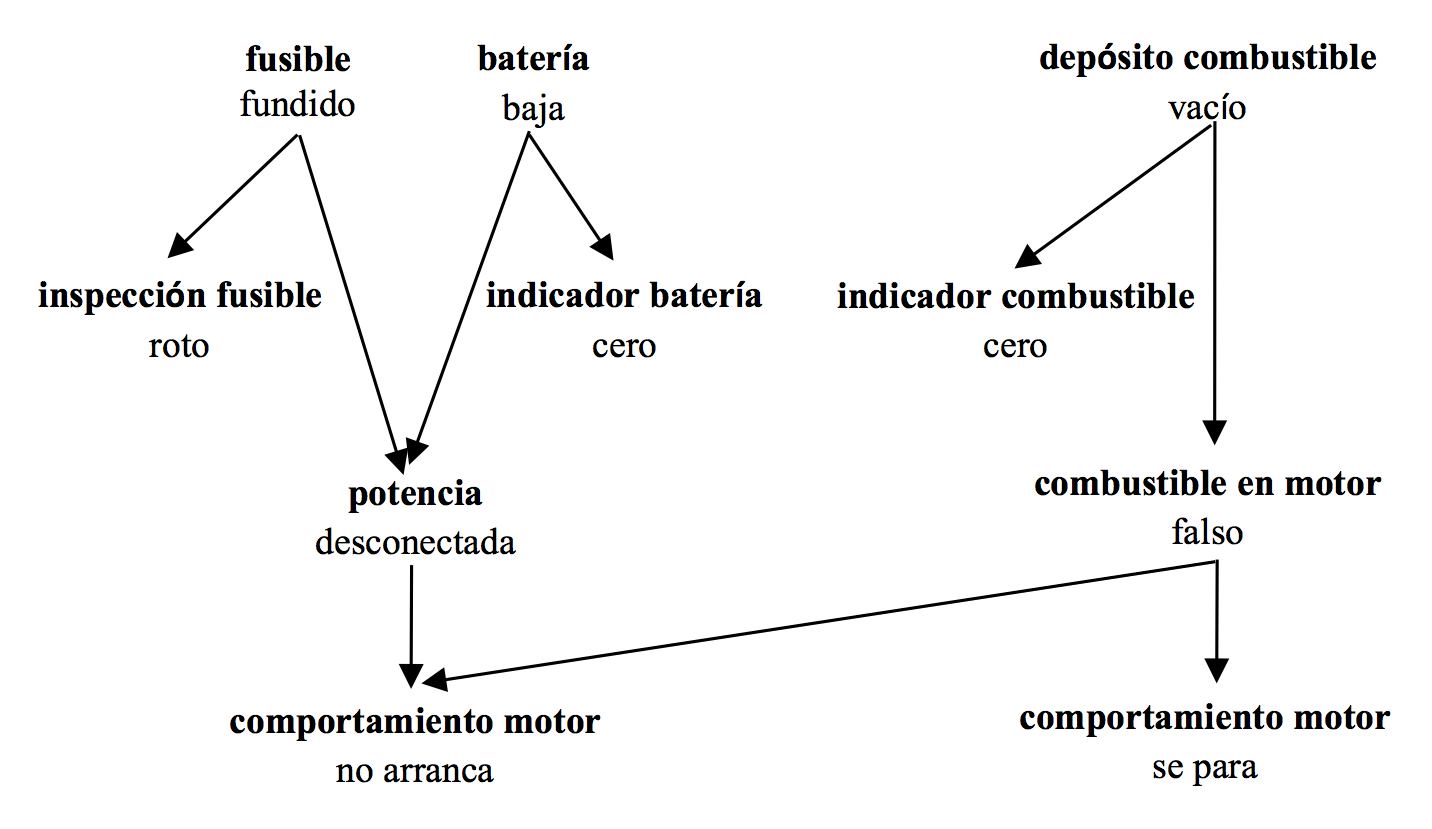
\includegraphics[width=0.75\textwidth]{exercise-3-network}
		\end{center}
	\end{figure}

    \section{La figura muestra un fragmento de una red causal que modela conocimiento del dominio para la tarea de diagnosis en el dominio de los automóviles. La red asocia posibles causas de fallo (fusible fundido, batería baja o depósito de combustible vacío) con estados intermedios (potencia, combustible en motor y síntomas comportamiento motor, inspección fusible, indicador batería...) Se puede observar que la red refleja la dirección causal: la causa "Depósito de combustible vacío" tiene como efecto "Combustible en motor falso" que a su vez es causa de "Comportamiento motor se para".}

        \paragraph{}
		Lorem ipsum dolor sit amet, consectetur adipisicing elit, sed do eiusmod tempor incididunt ut labore et dolore magna aliqua. Ut enim ad minim veniam, quis nostrud exercitation ullamco laboris nisi ut aliquip ex ea commodo consequat. Duis aute irure dolor in reprehenderit in voluptate velit esse cillum dolore eu fugiat nulla pariatur. Excepteur sint occaecat cupidatat non proident, sunt in culpa qui officia deserunt mollit anim id est laborum.


	\begin{figure}[H]
		\begin{center}
			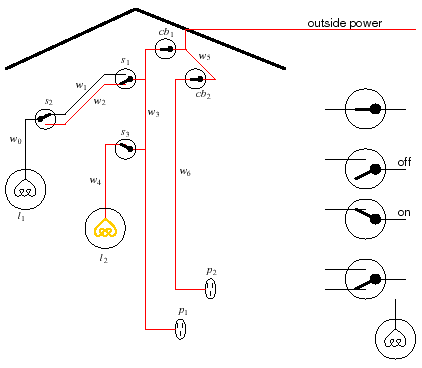
\includegraphics[width=0.6\textwidth]{diagnostic-assistant}
		\end{center}
	\end{figure}

	\section{Considerar el asistente al diagnostico propuesto por Pool y Mackworth}

		\paragraph{}
		Lorem ipsum dolor sit amet, consectetur adipisicing elit, sed do eiusmod tempor incididunt ut labore et dolore magna aliqua. Ut enim ad minim veniam, quis nostrud exercitation ullamco laboris nisi ut aliquip ex ea commodo consequat. Duis aute irure dolor in reprehenderit in voluptate velit esse cillum dolore eu fugiat nulla pariatur. Excepteur sint occaecat cupidatat non proident, sunt in culpa qui officia deserunt mollit anim id est laborum.

\end{document}
